%
%
\documentclass[10pt,a4paper,oneside]{book}

%Hello there. Don't know what to do?
	%Search for the %? and fix/add stuff.
	%Check zapiski 2007, your notes and your memory and fix/add stuff
	%kul knjige imajo quote na začetku poglavij

\usepackage[slovene]{babel}
\usepackage[utf8x]{inputenc}
\usepackage[fleqn]{amsmath}%fleqn - levo zamaknjene enačbe
\usepackage{amsfonts}
\usepackage{amssymb}
\usepackage{makeidx}
\usepackage{graphicx}
\usepackage[x11names, rgb]{xcolor}
\usepackage{tikz}
\usetikzlibrary{automata,snakes,arrows,shapes,decorations.text}

\usepackage{torstyle}
%?this feels too much like CSS hacks :(
%torstlye predloge:
%Definicija \Def{}
%Primer \Primer{}
%Prirejen itemize \begin{items}
\hypersetup{pdftitle={Teoretične osnove računalništva}}

\begin{document}
\begin{titlepage}
\begin{center}
\ \\[1cm]
{\Huge Teoretične osnove računalništva}\\[5pt]
{\LARGE Zapiski predavanj 2010/2011}\\[15pt]
{\large \today}\\[2.5cm]
\begin{center}%?is it too big? :P
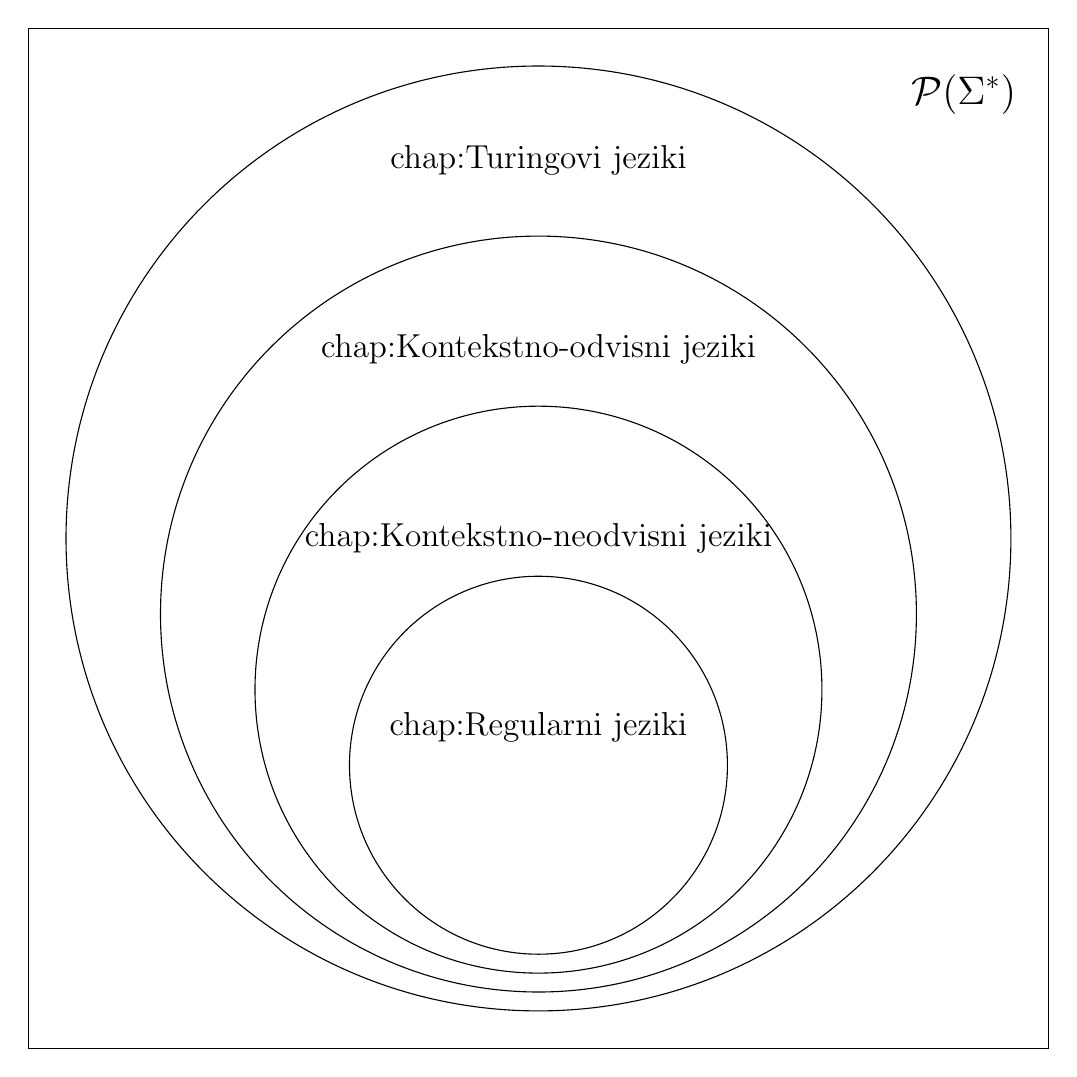
\begin{tikzpicture}[scale=1.2]
	\draw (-5.4cm,-5.4cm) rectangle (5.4cm,5.4cm);
	\node at (4.5cm,4.7cm) {\Large $\mathcal{P}(\Sigma^*)$};%sva šla vprašat slivnika... ker \Sigma^* znajo že RJ opisat, samo ne vseh možnih ;)

	\draw (0cm,0cm) circle (5cm);
	\node at (0,4cm) {\large \nameref{chap:Turingovi jeziki}};

	\draw (0cm,-0.8cm) circle (4cm);
	\node at (0,2cm) {\large \nameref{chap:Kontekstno-odvisni jeziki}};

	\draw (0cm,-1.6cm) circle (3cm);
	\node at (0,0cm) {\large \nameref{chap:Kontekstno-neodvisni jeziki}};

	\draw (0cm,-2.4cm) circle (2cm);
	\node at (0,-2cm) {\large \nameref{chap:Regularni jeziki}};
\end{tikzpicture}
\end{center}

\vfill
\parbox{7.5cm}{
\begin{center}

\includegraphics[width=0.15\textwidth]{./CC}\\[6pt]

This work is licensed under a Creative Commons Attribution-NonCommercial-ShareAlike 3.0 Unported License
\end{center}
}

\end{center}
\end{titlepage}
\tableofcontents
\pagebreak
%\newpage
%\section{Notacija}
%\begin{itemize}
%	\item[Množice:] Označimo z velikimi tiskanimi črkami. Podamo jih lahko na naslednje načine\\
%	$ A = \{ a_1, a_1, a_3, \ldots \} $ - naštevanje elementov\\
%	$ B = \{ n | \ \mbox{pravilo za n} \} \ $ - opis elementov
%\end{itemize}

\pagebreak
\chapter{Uvod}
\section{Matematične osnove}
\subsection{Dokazovanje}
\subsubsection{Dokaz s konstrukcijo}
Dokaz obstoja nekega matematičnega objekta je to, da nam ga uspe sestaviti.

\begin{primeri}
\item Za vsak $n>4$, obstaja dvojiško drevo, ki ima natanko $3$ liste.
%?manjka dokaz in slika
\item $| \mathbb{R} | = | [0,1) |$.\\
	\begin{items}
	\item Množici imata enako moč, kadar med njima obstaja bijektivna preslikava.
	\item Vsako realno število $r$ lahko zapišemo kot:
	\[ r=\pm d_1 d_2 \cdots d_n . \overline{d_1}\overline{d_2} \cdots \overline{d_m} \cdots;\ d_1 \neq 0 \]
	\item Definiramo preslikavo:
	\[ \mathbb{R}\rightarrow [0,1): r \rightarrow 0.s\overline{d_1} d_{n} \overline{d_2} d_{n-1} \cdots \overline{d_{n-1}} d_2 \overline{d_n} d_1 \overline{d_{n+1}} 0\overline{d_{n+2}} 0 \cdots \]
	kjer $s$ določa predznak ($s=0$, če $r \ge 0$ in $s=1$, sicer).
	\item Vidimo:
		\begin{items}
		\item $|\mathbb{R}|\le |[0,1)|$, %?(ker se $0.2$ ne da preslikati v $\mathbb{R}$)??
		\item $|\mathbb{R}|\ge |[0,1)|$, ker velja $[0,1) \subset \mathbb{R}$
		\end{items}
	\item Iz tega lahko sklepamo, da velja $|\mathbb{R}|=|[0,1)|$
	\end{items}
\end{primeri}
	
\subsubsection{Dokaz z indukcijo}
Če je množica induktivni razred%\footnote{Glej slovarček na koncu.}
, lahko z matematično indukcijo dokazujemo neko lastnost članov množice. Induktivni razred $I$ sestavlja:
\begin{items}
\item Baza indukcije - najbolj osnovna množica elementov (osnovni razred)
\item Pravila generiranja - kako iz elementov baze gradimo nove elemente (množico)
\end{items}
\begin{primeri}
\item Induktivni razred naravnih števil $(\mathbb{N})$
	\begin{items}
	\item Baza: $1 \in \mathbb{N}$ 
	\item Pravila generiranja: $n \in \mathbb{N} \Longrightarrow n+1 \in \mathbb{N} $
	\end{items}
\item \fnurl{Hilbertove krivulje}{http://en.wikipedia.org/wiki/Hilbert_curve}
\end{primeri}

\subsubsection{Dokaz s protislovjem}
Vzamemo nasprotno trditev, od tiste, ki jo želimo preveriti in pokažemo, da to vodi v protislovje.

\begin{primeri}
\item Praštevil je končno mnogo.
	\begin{items}
	\item Predpostavimo, da poznamo vsa praštevila:\\
		$P = \{2,3,5,...,p\}$, kjer je $p$ zadnje praštevilo 
	\item Po definiciji obstajajo le praštevila in sestavljena števila (to so taka, ki jih lahko razstavimo na prafaktorje). 
	\item Če pomnožimo vsa znana praštevila iz $P$ in prištejemo $1$ dobimo število, ki se ga ne da razstaviti na prafaktorje iz množice $P$:\\
		$q = 2 * 3 * 5 * ... * p + 1$
	\item Torej je $q$ ali praštevilo (ker ni sestavljeno), ali pa število, sestavljeno iz prafaktorjev, ki jih ni v množici $P$.
	\item Oboje kaže na to, da v množici $P$ nimamo vseh praštevil, ter, da to velja za vsako končno množico praštevil.
	\end{items}
\item $\sqrt[3]{2}$ je racionalno število.
	\begin{items}
	\item Če je $\sqrt[3]{2}$ racionalno število, ga je moč zapisati kot ulomek $\frac{a}{b}$.
	\item Predpostavimo, da je ulomek $\frac{a}{b}$ okrajšan (torej, da velja: $GCD(a,b)=1$):
		\begin{align*}
		\sqrt[3]{2} &= \frac{a}{b}\\
		2 &= \left( \frac{a}{b} \right)^3\\
		2b^3 &= a^3
		\end{align*}
	\item Opazimo, da je $a$ sodo število, torej lahko pišemo $a = 2k$:
		\begin{align*}
		2b &= \left( 2k\right)^3\\
		2b &= 8k\\
		b &= 4k
		\end{align*}
	\item Ker se je pokazalo, da je tudi $b$ sodo število, $GCD(a,b)=1$ ne more držati, torej smo prišli v protislovje in s tem dokazali, da $\sqrt[3]{2}$ ni racionalno število.
	\end{items}
\end{primeri}

\pagebreak
\chapter{Regularni jeziki}\label{chap:Regularni jeziki}

\section{Uvod}
\subsection{Uporabljene oznake}
\begin{items}
\item $a$ - znak ali simbol (niz dolžine 1)
\item $\Sigma$ - abeceda (končna neprazna množica znakov)
\item $w$ - niz ali beseda (poljubno končno zaporedje znakov $w_1w_2 \ldots w_n$)
\item $|w|$ - dolžina niza
\item $\varepsilon$ - prazen niz, $|w|=0$
\item $\Sigma^*$ - vsi možni nizi abecede
\end{items}


\subsection{Operacije nad regularnimi jeziki}
\begin{items}
\item Stik
	\begin{items}
	\item Stik nizov:
		\begin{align*}
		w  &= w_1 w_2 \dots w_n\\
		x  &= x_1 x_2 \dots x_m\\
		wx &= w_1 w_2 \dots w_n x_1 x_2 \dots x_m
		\end{align*}
	\item Stik množic:
		\begin{align*} 
		A & = \{ w_1 ,\ w_2 ,\ \dots ,\ w_n \} \\ 
		B & = \{ x_1 ,\ x_2 ,\ \dots ,\ x_m \} \\ 
		A \cdot B & = \{ w_ix_j \ | \ w_i \in A \ \wedge \ x_i \in B \}
		\end{align*} 
	\end{items}
\item Potenciranje
	\begin{align*} 
	A^0 & = \{ \varepsilon \} \\
	A^k & = A \cdot A \cdot \ldots \cdot A \ = \ \bigcirc_{i=1}^{k} A \\
	\end{align*}
\item Iteracija
	\begin{align*} 
	A^* &= A^0 \cup A^1 \cup A^2 \cdots  \ = \ \bigcup_{i=0}^{ \infty } A^i
	\end{align*} 		
\end{items}

\pagebreak
\section{Regularni izrazi}\label{sec:RI}
\Def{Imamo tri osnovne izraze:
	\begin{items}
	\item $\underline{\emptyset}$ je opisuje prazen jezik $ L(\underline{\emptyset})= \{ \}$
	\item $\underline{ \varepsilon }$ opisuje jezik $L(\underline{ \varepsilon })= \{ \varepsilon\}$
	\item $\underline{a}$ opisuje jezik $L( \underline{a} ) = \{ a \},\ a \in \Sigma$
	\end{items}
	In tri pravila za generiranje sestavljenih izrazov:
	\begin{items}
	\item $(r_1 + r_2)$ opisuje unijo jezikov $L(r_1 + r_2) = L(r_1) \bigcup L( r_2)$
	\item $(r_1\ r_2)$ opisuje stik jezikov $L(r_1\ r_2) = L(r_1)\cdot L( r_2)$
	\item $(r^*)$ opisuje iteracijo jezika $(L(r))^*$
	\end{items}
}
\begin{primeri}
\item Opiši vse nize, ki se končajo z nizom $00$ v abecedi $\Sigma = \{ 0,1 \}$.
	\[ r = (0+1)^*00 \]
	\item Opiši vse nize, pri katerih so vsi $a$-ji pred $b$-ji in vsi $b$-ji pred $c$-ji v abecedi $\Sigma = \{ a,b,c \}$.
		\[ a^*b^*c^* \]
	\item Opiši vse nize, ki vsebujejo vsaj dva niza '$aa$', ki se ne prekrivata v abecedi $\Sigma = \{ a,b,c \}$.
		\[ (a+b+c)^* aa (a+b+c)^* aa (a+b+c)^* \]
	\item Opiši vse nize, ki vsebuje vsaj dva niza '$aa$' ki se lahko prekrivata v abecedi $\Sigma = \{ a,b,c \}$
		\[ (a+b+c)^* aa (a+b+c)^* aa (a+b+c)^* + (a+b+c)^* aaa (a+b+c)^* \]
	\item Opiši vse nize, ki ne vsebujejo niza $11$ v abecedi $\Sigma = \{ 0,1 \}$
		\[ (\varepsilon  + 1 )(0^*01)^* 0^*	\]
		\[ (\varepsilon  + 1 )(0^* + 01)^* \]
	\item S slovensko abecedo opiši besedo "Ljubljana" v vseh sklonih in vseh mešanicah velikih in malih črk.
		\[ (L+l)(J+j)(U+u)(B+b)(L+l)(J+j)(A+a)(N+n)( (A+a)(O+o)(E+e)(I+i) ) \]
		Koliko različnih nizov opišemo s tem regularnim izrazom?\\
		\[ 2^8 \cdot 2^3 = 2^{11} \mbox{ nizov} \]
\end{primeri}

\section{Končni avtomati}\label{sec:KA}
\subsection{Nedeterministični končni avtomati z $\varepsilon$-prehodi }
\Def{$\varepsilon$NKA je definiran kot peterka $M = \langle Q, \Sigma, \delta ,q_0 , F \rangle$, kjer je:
	\begin{items}
	\item $ Q $ - končna množica stanj
	\item $ \Sigma $ - vhodna abeceda
	\item $ \delta $ - funkcija prehodov, $\delta : Q \times (\Sigma \cup \{\varepsilon\}) \rightarrow 2^Q$
	\item $ q_0 $ - začetno stanje
	\item $ F $ - množica končnih stanj
	\end{items}
}
%?razlaga potenčne množice bi šla lahko nekam med mat. osnove... imam še en kup stvari o teoriji množic nekje. Drugač je pa kul - epsilon-closure je že napol opisan :)
$2^Q=P(Q)$ je tu potenčna množica stanj avtomata. To pomeni da je so v $2^Q$ vse možne kombinacije stanj. Recimo da se nahajamo v stanju A, potem nas funkcija prehodov $ \delta $ pripelje v vsa mozna stanja do katerih pridemo iz $A$ z določenim znakom abecede in z vsemi $ \varepsilon $ prehodi, naprimer $ \{ A_1,A2, \ldots , A_n \}$. Tukaj je množica stanj $ \{ A_1,A2, \ldots , A_n \} $ element potenčne množice $P(Q)$

\subsection{Nedeterministični končni avtomati}
\Def{NKA je definiran kot peterka $M = \langle Q, \Sigma, \delta, q_0, F \rangle$, kjer je:
	\begin{items}
	\item $ Q $ - končna množica stanj
	\item $ \Sigma $ - vhodna abeceda
	\item $ \delta $ - funkcija prehodov $\delta : Q \times \Sigma \rightarrow 2^{Q}$
	\item $ q_0 $ - začetno stanje
	\item $ F $ - množica končnih stanj
	\end{items}		
}
\Def{Funkcija $\varepsilon$-closure($q$) nam pove, do katerih stanj lahko pridemo iz stanja $q$ po $\varepsilon$ prehodih.\\
	$\varepsilon$-closure($q$)$ = \{ q_k\ |\ \exists q_1, q_2, \dots q_n \in Q,\ q=q_1 \wedge q_i \in \delta(q_{i-1}, \varepsilon) \}$
}
\Def{Posplošena funkcija prehodov $\hat\delta$ nam pove, do katerega stanja pridemo po nekem nizu.\\
	$\hat\delta(q, \varepsilon) = \varepsilon$-closure($q$)\\
	$\hat\delta(q, a) = \delta(q, a)$\\
	$\hat\delta(q, wa) = \varepsilon$-closure($\{ q''\ |\ q' \in \hat\delta(q, w) \wedge q'' \in \delta(q', a) \})$
}

\subsection{Deterministični končni avtomat}
\Def{DKA je definiran kot petorka $M = \langle Q, \Sigma, \delta, q_0, F \rangle$, kjer je:
	\begin{items}
	\item $ Q $ - končna množica stanj
	\item $ \Sigma $ - vhodna abeceda
	\item $ \delta $ - funkcija prehodov, $\delta : Q \times \Sigma \rightarrow Q$
	\item $ q_0 $ - začetno stanje
	\item $ F $ - množica končnih stanj
	\end{items}	
}

\subsection{Jeziki končnih avtomatov}
\Def{Jezik $\varepsilon$NKA ter NKA je definiran kot:
	\begin{equation*}
	L=\{ w\ |\ \hat\delta(q_0, w) \cap F \neq \emptyset \}
	\end{equation*}
	kjer je $\hat\delta(q,w)$ posplošena funkcija prehodov v večih korakih.}%?Y you no define \varepsilon closure?
\Def{Jezik DKA je definiran kot:
	\begin{equation*}
	L=\{ w\ |\ \hat\delta(q_0, w) \in F \}
	\end{equation*}
}
Definicije želijo povedati, da so v jeziku točno tisti nizi, po katerih je iz začetnega stanja mogoče priti do nekega končnega stanja.

\section{Levo in desno-regularne gramatike}\label{sec:LG}
\Def{Regularna gramatika je definirana kot četvorček $G=\langle V,T,P,S \rangle$, kjer je:%?or is it NTPS?
\begin{items}
\item V - množica spremenljivk oz. vmesnih simbolov, $V \subseteq \Sigma$
\item T - množica znakov oz. končnih simbolov, $T \subset \Sigma$
\item P - množica produkcij, $\left[\alpha_1 \rightarrow \alpha_2 \right]$%? se da vse definirat tuki?
\item S - začetni simbol, $S \in V$
\end{items}
Pri tem pa regularne gramatike ločimo na levo in desno-regularne.
\begin{items}
\item Pri levih so produkcije $P \subset V \times ((V \cup \{\varepsilon\})\cdot T^*)$
\item Pri desnih so produkcije $P \subset V \times (T^* \cdot (V \cup \{\varepsilon\}))$
\end{items}
 }
To pomeni, da imamo pri levo-regularnih gramatikah vmesne simbole lahko le na skrajni levi, pri desno-regularnih pa le na desni.

\section{Jezik regularnih jezikov}
%?tu bi pasal dokazi :)
\Def{Jezik ki ga opisuje poljubni regularni izraz, končni avtomat, levo ali desno-linearna gramatika, je regularni jezik.}
Regularni jeziki ne vsebujejo informacije o prejšnjih znakih vhodnega niza in se z njimi ne da opisati poljubnega jezika. (za postopke dokazovanja regularnosti glej \ref{sec:Dokazovanje za RJ}).
\begin{primeri}
	%\item $\Sigma^* $ je regularni izraz %?wrong... jezik je nujno strogi subset \sigma*... ker ni dovolj močnega modela za opis vseh možnih nizov
	\item $L =\{ \}$ - prazen jezik
	\item $L = \{ \varepsilon \}$ - jezik, ki vsebuje $\varepsilon$ (ni prazen)
	\item $L = \{ a, aa, ab \}$ - jezik, ki vsebuje nize "a, aa, ab"
	\item $L = \{ 0^n 1^n \ | \ n \geqslant 0 \} $ - \underline{ni} regularni jezik, saj si poljubnega števila $n$ ne moremo zapomniti.
\end{primeri}

\section{Ohranjanje regularnosti jezikov}
Regularnost jezika že po definiciji ohranjajo operacije:
\begin{items}
\item $L_1 \cup L_2$ - unija 
\item $L_1 \cdot L_2$ - stik 
\item $L^*$ - iteracija
\end{items}
Obstajajo postopki za konstrukcijo, ki kažejo, da regularnost ohranjajo tudi:
\begin{items}
\item $L_1 \cap L_2$ - presek\\
	Iz avtomatov za $L_1$ in $L_2$ zgradimo t.i. produktni avtomat:
		\begin{align*}
			M_{L_1} &= \{ Q_1, \Sigma, \delta_1, q_{1_0}, F_1 \}\\
			M_{L_2} &= \{ Q_2, \Sigma, \delta_2, q_{2_0}, F_2 \}\\
			M_{L_1}*M_{L_2} &= \{ Q_1 \times Q_2, \Sigma, \delta_*, \langle q_{1_0}, q_{2_0} \rangle, F_1 \times F_2 \}
		\end{align*}
	Namesto stanj dobimo pare stanj in moramo preveriti v kateri par pridemo, če gledamo oba stara avtomata, končna pa so tista stanja, ki so končna v obeh starih avtomatih.
	\[ \delta_*(\langle q_1, q_2 \rangle, a) = \langle \delta_1(q_1, a), \delta_2(q_2, a)\rangle \]
\item $L^R$ - obrat oz. reverz\\
	Obrnemo vse povezave, ustvarimo novo začetno stanje, ki gre po $\varepsilon$ v stara končna, staro začetno stanje pa postane edino končno stanje.
\end{items}
Regularnost ohranjajo tudi vse operacije, ki so sestavljene iz zgoraj naštetih:
\begin{items}
\item $L_1 \setminus L_2 = L_1 \cap \overline L_2$ - razlika
\item $\overline{L} = \Sigma^* \setminus L$ - komplement
\item $L_1 \underline\vee L_2 = (L_1 \cup L_2) \setminus (L_1 \cap L_2)$ - ekskluzivni ali 
\end{items}

\section{Prevedba med modeli regularnih jezikov}%?lame naslov, fixme
Regularni izrazi, regularne gramatike in končni avtomati so enako močni modeli in je mogoče pretvarjati med njimi. V tem odseku bomo predstavili naslednje prevedbe:\\[12pt]%?ustrezno dopolni :)
\begin{center}
\begin{tikzpicture}[>=latex',/tikz/initial text=""]
	\node (RI)   at (0bp,0bp)   {RI};
	\node (eNKA) at (75bp,0bp)  {$\varepsilon$NKA};
	\node (NKA)  at (150bp,0bp) {NKA};
	\node (DKA)  at (225bp,0bp) {DKA};
	\node (DLG)  at (300bp,0bp) {DLG};
	\node (LLG)  at (375bp,0bp) {LLG};

	\draw [bend left,->]  (DKA) to node[auto] {\ref{KA-RI}} (RI);
\end{tikzpicture}
\end{center}

	%nekako tako mam v lanskih vajah, vrjetno mam letos bl prov :)
	%ps. lanske vaje so ful ugly, tko d si nism kj velik pomagov
	%\subsubsection{KA $\rightarrow$ DLG}
	%\subsubsection{DLG $\rightarrow$ KA}
	%\subsubsection{KA $\rightarrow$ RI}
	%\subsubsection{NKA $\rightarrow$ DKA}
	%\subsubsection{$\varepsilon$-NKA $\rightarrow$ NKA}
	%\subsubsection{RI $\rightarrow$ $\varepsilon$-NKA}

\subsection{Končni avtomat $\rightarrow$ Regularni izraz}\label{KA-RI}
Končni avtomat v regularni izraz prevedemo po metodi z eliminacijo. Pri tej metodi izberemo neko vozlišče za eliminacijo, nato pa njegove sosede povežemo med seboj, tako, da na nove povezave zapišemo regularne izraze, ki opisujejo dogajanje v tistem vozlišču. Eliminacijo ponavljamo, dokler nam v avtomatu ne ostanta le dve stanji, nato pa za končni zapis uporabimo naslednji recept:
\br
Na povezavah avtomata imamo zapisane regularne izraze $R,S,Q$ in $T$,\\
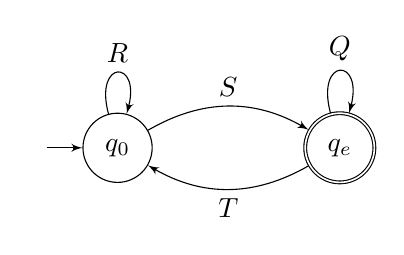
\begin{tikzpicture}[>=latex',/tikz/initial text=""]
	\node (q0) at (0bp,0bp)  [state, initial]   {$q_0$};
	\node (q1) at (80bp,0bp) [state, accepting] {$q_e$};

	\draw [loop above,->] (q0) to node[auto] {$R$} (q0);
	\draw [bend left,->]  (q0) to node[auto] {$S$} (q1);
	\draw [bend left,->]  (q1) to node[auto] {$T$} (q0);
	\draw [loop above,->] (q1) to node[auto] {$Q$} (q1);
\end{tikzpicture}
\\
ki jih prepišemo v en sam regularni izraz oblike:
\[ (R+SQ^*T)^*SQ^* \]

\begin{primeri}
\item Zapiši DKA za preverjanje deljivosti s 3 v binarnem sistemu? Zapiši še regularni izraz.\\
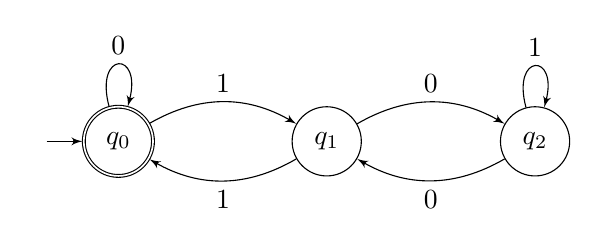
\begin{tikzpicture}[>=latex',/tikz/initial text=""]
	\node (q0) at (0bp,0bp)   [state, initial, accepting] {$q_0$};
	\node (q1) at (75bp,0bp)  [state]                     {$q_1$};
	\node (q2) at (150bp,0bp) [state]                     {$q_2$};

	\draw [loop above,->] (q0) to node[auto] {$0$} (q0);
	\draw [bend left,->]  (q0) to node[auto] {$1$} (q1);
	\draw [bend left,->]  (q1) to node[auto] {$1$} (q0);
	\draw [bend left,->]  (q1) to node[auto] {$0$} (q2);
	\draw [bend left,->]  (q2) to node[auto] {$0$} (q1);
 	\draw [loop above,->] (q2) to node[auto] {$1$} (q2);
\end{tikzpicture}
\ \\
Regularni izraz dobimo po postopku iz \ref{KA-RI}:
\[ (0+1(01^*0)^*1)^* \]
\end{primeri}

\section{Dokazovanje regularnosti jezika}\label{sec:Dokazovanje RJ}
%Dostikrat hočemo sestaviti regularen izraz za določen jezik in niti ne vemo ali je regularen izraz sploh regularen ali ne. Za to imamo nekaj metod za dokazovanje regularnosti jezika.%?false... ne moreš sestavit regularnega izraza, ki ni regularen :)
Kadar ugotavljamo, ali je nek jezik regularen, to lahko naredimo na več načinov:
\begin{items}
\item Pokažemo da je regularen:
	\begin{items}
	\item Jezik skonstruiramo v enem izmed modelov, ki sprejemajo regularne jezike:
		\begin{items}
		\item \nameref{sec:KA}
		\item \nameref{sec:RI}
		\item \nameref{sec:LG}
		\end{items}
	\end{items}
\item Dokažemo da ni regularen:
	\begin{items}
	\item Z uporabo leme o napihovanju za regularne jezike (glej \ref{sec:Lema za RJ})
	\item Pokažemo, da jezik ne spada niti v nek širši razred jezikov:
		\begin{items}
		\item Dokažemo, da ni kontekstno-neodvisen (glej \ref{sec:Dokazovanje KNJ})
		\end{items}
	\end{items}
\end{items}
%?what is this, I don't even :D
%Opozorilo: Če zapišemo regularni izraz za jezik, ali naredimo končni avtomat, moramo dobro preveriti da ne obstaja kakšen protiprimer. Torej beseda ki je v jeziku in jo končni avtomat ali regularni izraz ne sprejme, ali obratno.\\
%Če nam ne uspe dokaza (da je ali da ni regularni jezik) do konca speljati, to ne moremo vzeti kot dokaz da ravno nasprotno drži. Velja da v takem primeru še nič ne vemo o regularnosti jezika.

\subsection{Lema o napihovanju za regularne jezike}\label{sec:Lema za RJ}
Lemo o napihovanju za regularne jezike uporabljamo za dokazovanje, da nek jezik ne spada v razred regularnih jezikov. 
\Def{Za vsak regularni jezik obstaja neka konstanta $n$, taka, da lahko vsako besedo $w$ iz jezika, daljšo od $n$, razbijemo na tri dele:
	\[ w=u\ v\ z \]
	Pri čemer velja:
	\begin{items}
	\item $|uv| \leq n$
	\item $|v| > 0$
	\item $uv^iz \in L,\ \forall i \geq 0$ (napihovanje)
	\end{items}
}
Ker dokazujemo da jezik ni regularen, moramo torej najti neko besedo, za katero pri napihovanju ne ostanemo znotraj jezika. Če nam tega z izbrano besedo ne uspe dokazati, še nismo dokazali da je jezik regularen -- edini pravi dokaz tega je konstrukcija jezika v enem izmed modelov, ki opisujejo regularne jezike.
\begin{center}
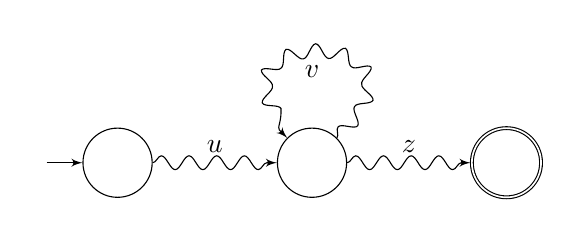
\begin{tikzpicture}[>=latex',/tikz/initial text=""]%scale=0.70, every state/.style={scale=0.70}]
	\node (q0) at (0bp,0bp)  [state, initial]   {};
	\node (q1) at (70bp,0bp) [state]            {};
	\node (q2) at (140bp,0bp) [state, accepting] {};

	\draw [decorate, decoration={snake},->]  (q0) to node[auto] {$u$} (q1);
	\draw [decorate, decoration={snake}, loop,->] (q1) to node[auto] {$v$} (q1);
	\draw [decorate, decoration={snake},->]  (q1) to node[auto] {$z$} (q2);
\end{tikzpicture}
\end{center}
Če zgornjo definicijo pogledamo v kontekstu končnih avtomatov, vidimo, da je $n$ gotovo večji od števila stanj, saj mora za napihovanje v avtomatu obstajati nek cikel, sicer bi bi veljalo $|v|=0$.

\chapter{Kontekstno-neodvisni jeziki}\label{chap:Kontekstno-neodvisni jeziki}
\section{Kontekstno-neodvisne gramatike}

\subsection{Chomskyeva normalna oblika}
\Def{Kontekstno-neodvisna gramatika je v Chomskyevi normalni obliki, kadar nima nekoristnih simbolov, ter so vse produkcije naslednjih dveh oblik:\\
	\[ A \rightarrow a \]
	\[ A \rightarrow BC \]
	\[ a \in T,\ \ B,C \in N \]
}
\subsection{Greibachina normalna oblika}
\Def{Kontekstno-neodvisna gramatika je v Greibachini normalni obliki, kadar so vse produkcije oblike:\\
	\[ A \rightarrow a\alpha\]
	\[ a \in T,\ \ \alpha \in N^* \]
}

\section{Skladovni avtomati}
\Def{Skladovni avtomat je definiran kot sedmerka $M=\langle Q, \Sigma, \Gamma, \delta, q_0, Z_0, F \rangle$, kjer je:
	\begin{items}
	\item $ Q $ - končna množica stanj
	\item $ \Sigma $ - vhodna abeceda
	\item $ \Gamma $ - skladovna abeceda
	\item $ \delta $ - funkcija prehodov, $\delta : Q \times (\Sigma \cup \{\varepsilon\}) \times \Gamma \rightarrow 2^{Q \times \Gamma^*}$%? zakaj U \varepsilon?
	\item $ q_0 $ - začetno stanje, $q_0 \in Q$
	\item $ Z_0 $ - začetni skladovni simbol, $Z_0 \in \Gamma$
	\item $ F $ - množica končnih stanj
	\end{items}
}
\subsection{Trenutni opis}
\Def{Trenutni opis je trojka $\langle q, w, \gamma \rangle \in Q \times \Sigma^* \times \Gamma^*$, pri čemer je $q$ trenutno stanje, $w$ preostanek vhodnega niza, ter $\gamma$ trenutna vsebina sklada}
\subsection{Relacija $\vdash$}
\Def{Relacija $\vdash$ nas pelje iz enega trenutnega opisa v drugega, če je ta prehod predviden v funkciji prehodov $\delta$:
	\[ \langle q, aw, Z\gamma \rangle \vdash \langle p, w, \gamma'\gamma \rangle \iff \langle p, \gamma' \rangle \in \delta(q,a,Z) \]
}
Uporabljamo tudi posplošeno relacijo $\vdash^*$, ki je ubistvu samo ena ali več-kratna uporaba relacije $\vdash$. Pove nam to, da pridemo iz enega trenutnega opisa do drugega, prek enega ali večih prehodov, pod pogojem, da vse vmesne prehode predvideva funkcija prehodov $\delta$.

\subsection{Jezik skladovnega avtomata}

\section{Dokazovanje kontekstne-neodvisnosti}\label{sec:Dokazovanje KNJ}
\subsection{Lema o napihovanju za kontekstno-neodvisne jezike}
\subsection{Ogdenova lema za kontekstno-neodvisne jezike}

%?appendix this:
%\chapter{Slovar}
%?zihr obstaja neki za to, sicer naredi definitions okolje
%\begin{items}
%\item Razred - razred je množica elementov, ki ga lahko podamo z naštevanjem elementov ali z opisom lastnosti (opisni ali konceptualni razredi)
%\end{items}

%----------------------------------------------------------------------
\chapter{Kontekstno-odvisni jeziki}\label{chap:Kontekstno-odvisni jeziki}
Prepoznajo jezik $L=\{ a^n b^n c^n | n>0 \}$, imajo gramatike s produkcijami oblike $AaB \rightarrow \alpha_1 a \beta_2$.

\chapter{Turingovi jeziki}\label{chap:Turingovi jeziki}
\section{Zgodovina}
%I've got 23 problems, but a bitch ain't one. -Hilbert, 1900
%\br
Leta 1900 je Nemški matematik David Hilbert objavil seznam triidvajsetih nerešenih problemov v matematiki. Eden izmed Hilbertovih problemov (deseti po vrsti), je vprašanje, ali obstaja postopek, po katerem ugotovimo rešljivost poljubne Diofantske enačbe -- torej, ali lahko ugotovimo, če ima polinom s celoštevilskimi koeficienti $P(x_1, x_2, \dots, x_n)=0$, celoštevilsko rešitev.
%?non-sequitur... vsaj dokler ne bo ogromno več zgodovine tu :)
Kljub temu, da je Emil Post že leta 1944 slutil, da je problem nerešljiv, je to dokončno dokazal rus Jurij Matijaševič šele leta 1970 v svojem doktorskem delu. Med reševanjem problema pa so se matematiki že prej začeli ukvarjati s formalizacijo pojma postopka oz. algoritma. Intuitivna definicija tega se glasi nekako tako:
\Def{Algoritem je zaporedje ukazov, s katerimi se v končnem številu korakov opravi neka naloga.}
Pri tem pa ostaja še kar nekaj odprtih vprašanj, npr.:
\begin{items}
\item Kakšni naj bodo ukazi? 
	\begin{items}
	\item Osnovni - algoritem ima veliko korakov
	\item Kompleksni - prezapleteni ukazi so že sami algoritmi
	\end{items}
\item Koliko ukazov naj bo?
	\begin{items}
	\item Končno - ali je s končno množico res mogoče rešiti vsako nalogo?
	\item Neskončno - kakšen izvajalec ukazov je sposoben izvršiti neskončno različnih ukazov?
	\end{items}
\item So ukazi zvezni ali diskretni?
\item V kakšnem pomnilniku so ukazi shranjeni?
	\begin{items}%?verjetno ista vprašanja kot pri št. ukazov?
	\item Končnem - ali s končnim zaporedjem ukazov res lahko mogoče rešimo vsako nalogo?
	\item Neskončnem - %?
	\end{items}
\end{items}
Nekateri zgodnji poskusi formalizacije pojma algoritma so:%? zgodovinsko zaporedje, letnice, imena modelov, moar info
\begin{items}
    \item GK (Kurt Gödel, Stephen Kleene) 
    \item HG (Jacques Herbrand, Kurt Gödel)
    %\item (Andrey Markov), %? sin Markova http://en.wikipedia.org/wiki/Andrey_Markov_(Soviet_mathematician)
    \item Produkcijski sistem (Emil Post), %? je to http://en.wikipedia.org/wiki/Tag_system? 1943?
    \item Lambda račun (Alonso Church, 1936)
    \item Turingov stroj (Alan Turing, 1936)
\end{items}

\pagebreak
\section{Turingovi stroji}
Turingov stroj se je uveljavil kot uporaben in preprost model računanja, ki zna izračunati vse kar se izračunati da (pod pogojem, da Church-Turingova teza drži). Alan Turing je svoj stroj izpeljal iz razmišljanja o tem, kako človek rešuje miselne probleme na papir. Pri tem je izbral tri sestavne dele:
\begin{items}
\item Nadzorno enoto (glava)
\item Čitalno okno (roka in vid)
\item Trak (papir)
\end{items}
V postopku formalizacije, pa je zaradi večje preprostosti, zahteval še, da je stroj sestavljen iz končno mnogo elementov, ter da deluje v diskretnih korakih.%?končno mnogo elementov? na kaj to cilja?

%?slika nadzorne enote, traku in okna

\Def{Turingov stroj je definiran kot sedmerka $M=\langle Q, \Sigma, \Gamma, \delta, q_0, B, F \rangle $, kjer je:
\begin{items}
	\item $Q$ končna množica stanj
	\item $\Sigma$ končna množica vhodnih simbolov, $Q \cap \Sigma = \emptyset$
	\item $\Gamma$ končna množica tračnih simbolov, $\Sigma \subset \Gamma$
	\item $\delta$ funkcija prehodov: $Q \times \Gamma \rightarrow Q \times \Gamma \times \{L,D\}$,\\ kjer $L$ in $D$ označujeta premik levo ali desno
	\item $q_0$ začetno stanje, $q_0 \in Q$
	\item $B$ prazen simbol, $B \in \Gamma$
	\item $F$ množica končnih stanj, $F \subseteq Q$ 
\end{items}}
Stroj deluje tako, da v vsakem koraku opravi naslednje:
\begin{items}
	\item preide v neko stanje
	\item zapiše nov simbol v celico, ki je pod oknom
	\item okno premakne eno celico levo ali desno
\end{items}

\subsection{Trenutni opis}
\Def{$TO = \Gamma^* \times Q \times \Gamma^*$ je množica vseh trenutnih opisov.\\
Nek trenutni opis $\langle \alpha_1, q, \alpha_2 \rangle$, ali krajše $\alpha_1\ q\ \alpha_2$ opisuje konfiguracijo Turingovega stroja.
%?slika TS z označenim \alpha_1, \alpha_2
\br
Iz $\alpha_1$ in $\alpha_2$, lahko razberemo:
\begin{items}
	\item če je $\alpha_1 = \varepsilon$, je okno skrajno levo
	\item če je $\alpha_2 = \varepsilon$, je okno nad $B$ in so naprej sami $B$-ji
\end{items}}

\subsection{Relacija $\vdash$}
\Def{Če sta $u,v$ trenutna opisa iz množice $TO$, ter $v$ neposredno sledi iz $u$ v enem koraku Turingovega stroja, tedaj pišemo $u \vdash v$.
\br
Naj bo $x_1 \dots x_{i-1}\ q\ x_i \dots x_n$ trenutni opis:
\begin{items}
\item če je $\delta(q,x_i) = \langle p,Y,D \rangle$:\\
$x_1 \dots x_{i-1}\ q\ x_i \dots x_n \vdash x_1 \dots x_{i-1}\ Y\ p\ x_{i+1} \dots x_n$
\item če je $\delta(q,x_i) = \langle p,Y,L \rangle$: 
	\begin{items}
	\item če je okno na robu ($i=1$), se Turingov stroj ustavi, ker je trak na levi omejen.
	\item če okno ni na robu ($i>1$), potem: $x_1 \dots x_{i-2} x_{i-1}\ q\ x_i \dots x_n \vdash x_1 \dots\ x_{i-2} p\ x_{i-1}\ Y\ x_{i+1} \dots x_n$
	\end{items}
\end{items}}
\subsection{Tranzitivna ovojnica $\vdash^*$ relacije $\vdash$}%?je pravi naslov?
\Def{$u \vdash^* v$, če obstaja tako zaporedje $x_i, (i \in [0, 1, \dots, k], k \geq 0)$, da velja $u=x_0, v=x_k$ in $x_0 \vdash x_1 \wedge x_1 \vdash x_2 \wedge \dots \wedge x_{k-1} \vdash x_k$
\br
Torej, trenutni opis $v$ sledi iz $u$, v $k$ korakih Turingovega stroja.}
\section{Jezik Turingovega stroja}
\Def{Jezik Turingovega stroja je definiran kot:
\begin{equation*}
L(M) = \{ w\ |\ w \in \Sigma^* \wedge q_0w \vdash^* w_1\ q\ w_2 \wedge w_1,w_2 \in \Gamma^* \wedge q \in F \}
\end{equation*}
}
%? slika z vhodno besedo na traku TS
Z besedami to pomeni, da je $L(M)$ množica besed $w \in \Sigma^*$, ki če jih damo na vhod stroju $M$, povzročijo, da se stroj $M$ v končno mnogo korakih znajde v končnem stanju.
\Def{Jezik $L$ je Turingov jezik, če obstaja Turingov stroj $M$, tak, da je $L = L(M)$.}
\subsection{Ugotavljanje pripadnosti besed Turingovemu jeziku}%?made one blockoftext from a lot of text. sm kj zgrešil?
Pri vprašanju ali je neka beseda v jeziku, Turingove jezike ločimo na:
\begin{items}
\item Odločljive - obstaja algoritem, s katerim se lahko za poljubno besedo odločimo, ali pripada jeziku.
\item Neodločljive - v splošnem ni algoritma, ki bi za poljubno vhodno besedo z DA ali NE odgovoril na vprašanje pripadnosti.
	\begin{items}
	\item če je odgovor DA, to ugotovimo v nekem končnem številu korakov.
	\item če je odgovor NE, pa ni nujno, da se bo stroj kdaj ustavil.
	\end{items}
\end{items}

%? slika venn.. x znotraj L kroga... v kvadratu

%?where does this go?
%Terminologija: re (recursively enumerable, Turing recognizable)%?semi-decidable? 
%Rekurzivni jezik (decidable)%?where does this go?

%? slika venn... odločljivi jeziki so znotraj Turingovih

\Primer{Zapiši Turingov stroj, ki sprejema jezik $L=\{0^n 1^n | n \geq 1\}$\\
	Skica izvajanja stroja:
	\begin{items}
	\item $0^{n}1^{n}$ - vhodna beseda
	\item $X0^{n-1}1^{n}$ - zamenjamo najbolj levo $0$ z $X$
	\item $X0^{n-1}Y1^{n-1}$ - premaknemo okno desno do najbolj leve $1$ in jo zamenjamo z $Y$
	\item $XX0^{n-2}Y1^{n-1}$\\ 
		$XX0^{n-2}YY1^{n-2}$ - ponovimo in vidimo, da bomo niz sprejeli, če je prave oblike.
	\end{items}
	Turingov stroj zapišemo kot $M=\langle Q,\Sigma,\Gamma,\delta,q_0,B,F \rangle$:
	\begin{items}
    \item $Q=\{ q_0,q_1,q_2,q_3,q_4 \}$
    \item $\Sigma = \{ 0,1 \}$
    \item $\Gamma = \{ 0,1,B,X,Y \}$
    \item $F = \{ q_4 \}$
    \item $\delta$ bomo definirali s tabelo
	\end{items}

    Pomen stanj:
    \begin{items}
    \item $q_0$ - začetno stanje in stanje pred zamenjavo 0 z X
    \item $q_1$ - premikanje desno do 1
    \item $q_2$ - zamenjava 1 z Y in premikanje levo do X
    \item $q_3$ - najde X in se premik desno
    \item $q_4$ - končno stanje
    \end{items}

    Tabela prehajanja stanj:\\
	\begin{center}
    \begin{tabular}{ c | c c c c c}
	& 0 & 1 & B & X & Y\\ \hline
	$x_0$& $\langle q_1,X,D\rangle$ & -- & -- & $\langle q_3,Y,D\rangle$ & --\\
	$x_1$& $\langle q_1,0,D\rangle$ & $\langle q_2,Y,L\rangle$ & -- & $\langle q_1,Y,D\rangle$ & --\\
	$x_2$& $\langle q_2,0,D\rangle$ & -- & $\langle q_0,X,D\rangle$ & $\langle q_2,Y,L\rangle$ & --\\
	$x_3$& -- & -- & -- & $\langle q_3,Y,D\rangle$ & $\langle q_4,B,D\rangle$\\
	$x_4$& -- & -- & -- & -- & --\\
	\end{tabular}
	\end{center}
	\br
	Izvajanje stroja s trenutnimi opisi:
	\[ q_0 0011 \vdash X q_1 011 \vdash X 0 q_1 11 \vdash X q_2 0 Y 1 \vdash \dots \]
}
%?zapiski 2007 imajo tu še nekaj o turingovih jezikih
\subsection{Turingov stroj kot računalnik funkcij}
Imamo Turingov stroj, ki ima na traku neko število ničel, ki predstavljajo pozitivna naravna števila, ločena z enicami:
	\[ 0^{i_1} 1 0^{i_2} 1  \dots 1 0^{i_k} \]
%?skupine ničel so i_1, i_2, ..., kjer so i naravna števila (mjbi i+1 ničel)  
%?slika TS z števili i_j na traku
Recimo, da se stroj po nekem številu korakov ustavi in ima na traku skupino ničel $0^m$, na levi in desni strani skupine pa same $B$-je. S tem je stroj lahko izračunal neko funkcijo
	\[ f^{(k)}:\mathbb{N}_+^k \rightarrow \mathbb{N}_+ \mbox{\ \ oz. \ \ } f(i_1, i_2, \dots, i_k) = m \]
%?slika TS s skupino ničel na traku
Funkcija $f$ ni nujno definirana za vsako $k$-terico iz $\mathbb{N}_+^k$, torej je parcialna funkcija, kadar pa je definirana povsod, pravimo da je totalna. Stroj se pri nedefiniranih $k$-tericah pač na neki točki ustavi in pri tem na traku ne pusti le ene skupine ničel, ali pa se sploh ne ustavi.
Isti turingov stroj hkrati računa več funkcij: $f^{(1)}, f^{(2)}, \dots f^{(k)}$.%?računa ali "lahko računa".. ne štekam ubistvu čist

\subsubsection{Parcialna rekurzivna funkcija}
\Def{Vsaka funkcija $f^{(k)}:\mathbb{N}_+^k \rightarrow \mathbb{N}$, ki jo lahko izračuna nek Turingov stroj, je parcialna rekurzivna funkcija. Če je $f^{(k)}$ definirana za vse $k$-terice, jo imenujemo totalna rekurzivna funkcija (včasih samo rekurzivna funkcija)}
Vse običajne aritmetične funkcije so parcialne ali celo totalne rekurzivne funkcije. V primerih si bomo pogledali nekaj primerov, tu pa jih nekaj naštejmo: $m+n,\ m*n,\ n!,\ 2^n,\ \lceil \log(n) \rceil,\ m^n,\ \dots$.
%so najdl primer, ki ne spada sem z diagonalizacijo
%na začetku so gledali totalne... pa so vidl da morajo parcialne
\begin{primeri}
\item
    Ali je $f(m,n)=m+n$ (parcialno) rekurzivna?\\
    Skica stroja, ki računa $m+n$:
    \begin{items}
    \item $0^m 1 0^m$ - vhodna beseda
    \item $B0^{m-1} 1 0^m$ - izbriši prvo ničlo
    \item $B0^{m+n}$ - premakni se do 1 in jo zamenjaj z 0
    \end{items}%?DN naredi cel stroj
\item
    Ali je $f(m,n)=m*n$ (parcialno) rekurzivna?\\
    Skica stroja, ki računa $m*n$:
    \begin{items}
    \item $0^m 1 0^n$ - vhodna beseda
    \item $0^m 1 0^n 1$ - premakni se na konec in zapiši 1 (ločnica za rezultat)
    \item $B 0^{m-1} 1 0^n 1$ - premakni se na začetek in izbriši 0
    \item $B 0^{m-1} 1 0^m 1 0^n$ - prekopiraj $n$ ničel za ločnico (in ničle)
    \item $B^{m} 1 0^m 1 0^{m*n}$ - ponavljaj tadva koraka, dokler ni več ničel pred prvo 1
    \item $B^{m+n+2}0^{m*n}$ - izbriši del, ki ne spada v rezultat 
    \end{items}%?naredi cel stroj
\end{primeri}

\subsection{Lažja konstrukcija Turingovih strojev}
Obstaja nekaj tehnik, ki poenostavijo in pohitrijo sestavljanje Turingovih strojev.%tu itak mislimo funkcije delta
\subsubsection{Nadzorna enota kot pomnilnik}
Vsako stanje stroja, je sestavljeno iz dveh delov -- stanja avtomata, ter shrambe za tračne znake. Novo množico stanj zapišemo kot $Q=K\times\Gamma$, kjer je $K$ stara množica stanj in $\Gamma$ tračna abeceda.
\Primer{Sestavi Turingov stroj za razpoznavanje besed, pri katerih se prvi znak ne ponovi:\\
	Stroj $M=\langle Q,\Sigma,\Gamma,\delta,q_0,B,F \rangle$ zapišemo kot:
	\begin{items}
	\item $M=\langle Q, \{0,1\}, \{0,1,B\}, \delta, \langle q_0, B \rangle, B, F \rangle$
	\item $Q=\{ q_0, q_1 \} \times \{0,1,B\} = \{ \langle q_0, 0\rangle , \langle q_0, 1\rangle , \langle q_0, B\rangle , \langle q_1, 0\rangle , \langle q_1, 1\rangle , \langle q_1, B\rangle\} $
	\item $F=\{ \langle q_1, B \rangle \}$
	\item $\delta$ zapišemo kot:
		\begin{items}
		\item Shrani prvi znak besede v stanje stroja:\\
			$\delta(\langle q_0, B\rangle, 0) = \langle\langle q_1, 0 \rangle, 0, D\rangle$\\
			$\delta(\langle q_0, B\rangle, 1) = \langle\langle q_1, 1 \rangle, 1, D\rangle$
		\item Premakni okno v desno do prvega znaka, enakega shranjenemu:\\
			$\delta(\langle q_1, 0\rangle, 1) = \langle\langle q_1, 0 \rangle, 1, D\rangle$\\
			$\delta(\langle q_1, 1\rangle, 0) = \langle\langle q_1, 1 \rangle, 0, D\rangle$
		\item Če prebereš $B$, pojdi v končno stanje:\\
			$\delta(\langle q_1, 0\rangle, B) = \langle\langle q_1, B \rangle, karkoli \rangle$\\
			$\delta(\langle q_1, 1\rangle, B) = \langle\langle q_1, B \rangle, karkoli \rangle$
		\item Sicer se ustavi. To dosežemo tako, da ne definiramo prehodov:\\
			$\delta(\langle q_1, 0\rangle, 0)$ in $\delta(\langle q_1, 1\rangle, 1)$
		\end{items}
	\end{items}
}
\subsubsection{Večsledni trak}
Na traku imamo več kot eno sled, kar pomeni, da s traku beremo $k$-terice tračnih znakov, kar zapišemo kot: $\Gamma=\Gamma_1\times\Gamma_2\times\dots\times\Gamma_k$.
\Primer{Sestavi Turingov stroj, ki preveri, ali je vhodno število praštevilo.\\
	Skica stroja:
	\begin{items}
	\item Trak ima tri sledi:
		\begin{items}
		\item na prvi sledi je vhodno število
		\item na drugi sledi je števec, ki na začetku hrani število 2
		\item tretjo sled uporabimo za delovno sled, na začetku je lahko prazna.
		\end{items}
	\item Stroj deluje tako:
		\begin{items}
		\item prepiši število s prve sledi na tretjo sled
		\item odštevaj število iz druge sledi od števila na tretji sledi
		\item če se odštevanje konča z 0, se ustavi (ni praštevilo)
		\item sicer število na drugi sledi povečaj za 1
		\item če je število na drugi sledi enako tistemu na prvi, sprejmemo (je praštevilo)
		\item sicer, ponovimo postopek
		\end{items}
	\end{items}
}
\subsubsection{Prestavljanje vsebine traku}
Recimo, da bi s traku radi vzeli nekaj zaporednih znakov tako, kot da bi jih izrezali iz traku in nato trak zlepili nazaj skupaj, izrezane simbole pa bi si pri tem seveda radi nekako zapomnili. Tudi to metodo realiziramo s pomočjo shrambe za tračne simbole v nadzorni enoti, a moramo pri tem paziti, da je funkcija prehodov pravilno napisana.
%?slika "guba"
%?slika nadzorna enota
\Primer{Sestavi Turingov stroj, ki premakne vsebino traku za 2 celici v desno.\\
	Skica stroja:
	\begin{items}
    \item $Q$ vsebuje stanja oblike: $\langle q, A_1, A_2 \rangle;\ q \in \{ q_1, q_2 \},\ A_1, A_2 \in \Gamma$
    \item $\Gamma$ poleg ostalih znakov, vsebuje še poseben znak $X$, ki označuje izpraznjeno celico na traku
	\item $F=\{ q_2 \}$
	\item $\delta$ zapišemo kot:
		\begin{items}
		\item Prva koraka -- zapomni si in izprazni prvi in drugi znak:\\
			$\delta(\langle q_1, B, B\rangle, A_1) = \langle\langle q_1, B, A_1 \rangle, X, D \rangle $\\
			$\delta(\langle q_1, B, A_1\rangle, A_2) = \langle\langle q_1, A_1, A_2 \rangle, X, D \rangle $
		\item Zapomni si nov znak in prvega iz shrambe zapiši na trak:\\
			$\delta(\langle q_1, A_i, A_{i+1}\rangle, A_{i+2}) = \langle\langle q_1, A_{i+1}, A_{i+2} \rangle, A_i, D \rangle $
		\item Zadnja koraka -- zapiši vsebino shrambe na trak:\\
			$\delta(\langle q_1, A_{n-1}, A_{n}\rangle, B) = \langle\langle q_1, A_{n}, B \rangle, A_{n-1}, D \rangle $\\
			$\delta(\langle q_1, A_{n}, B\rangle, B) = \langle\langle q_2, B, B \rangle, A_{n}, L \rangle $
		\end{items}
	\end{items}
}

\subsubsection{Podprogrami}
%?Imamo neka posebna stanja, ki signalizirajo vhod in izhod iz podprograma%?je tu govoril o dveh strojih?

%?tu je razlagal tisto neizračunljivo funkcijo nad matrikami. @zidar: poglej tor2-dodatno.pdf - tam govori o preroku

\end{document}